\documentclass{article}

\usepackage{tikz}
\usetikzlibrary{mindmap,trees}
\definecolor{tum_blue}{rgb} {0.00,0.40,0.74}
\definecolor{tum_lgray}{rgb}{0.85,0.85,0.86}
\definecolor{tum_lblue}{rgb}{0.39,0.63,0.78}
\begin{document}
\pagestyle{empty}
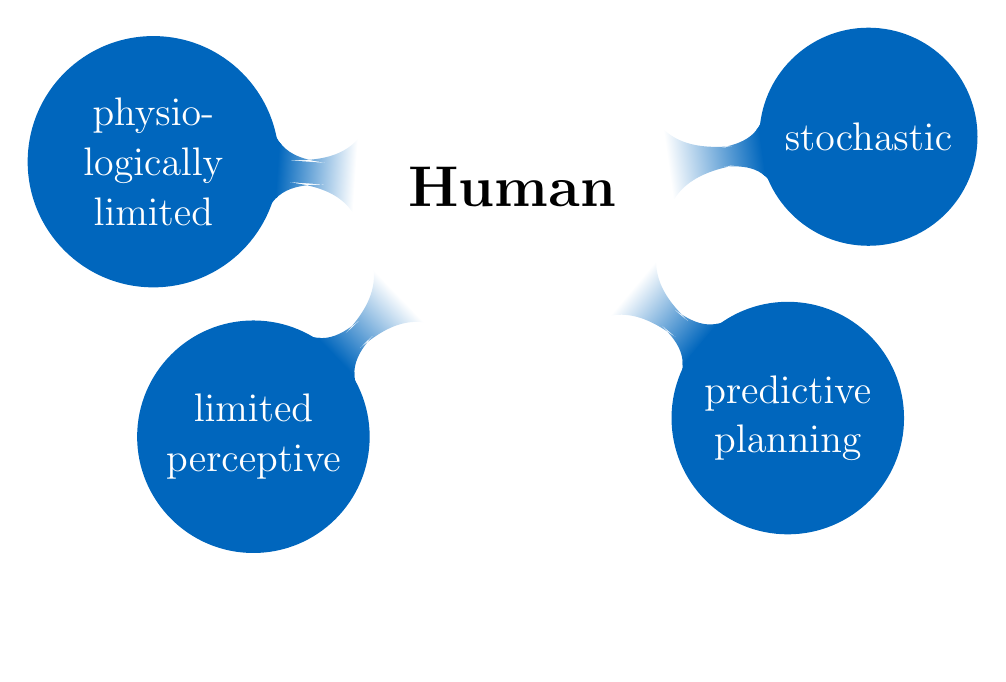
\begin{tikzpicture}
  \path[mindmap,concept color=white,text=white,
    every node/.style={font=\Large},
    root concept/.append style = {font=\huge\bfseries},
    level 1 concept/.append style={font=\Large,
      sibling angle=48,text width=7.7em,
    level distance=13em,inner sep=0pt},
     ]
    node[concept] {\huge\bfseries\color{black} Human}
    [clockwise from=8]
    %child[concept color=tum_blue] { node[concept] {error prone} }
    child[concept color=tum_blue] { node[concept] {stochastic}  }
    child[concept color=tum_blue] { node[concept] {predictive planning} }
    %    child[concept color=white] { node[concept] {} }
                child[concept color=black, opacity=0] { node[concept] {} }
    child[concept color=tum_blue] { node[concept] {limited perceptive} }
    child[concept color=tum_blue] { node[concept] {physio-logically limited} } ; 
    %child[concept color=tum_blue] { node[concept] {adaptive} };
\end{tikzpicture}\end{document}